170. \begin{figure}[ht!]
\center{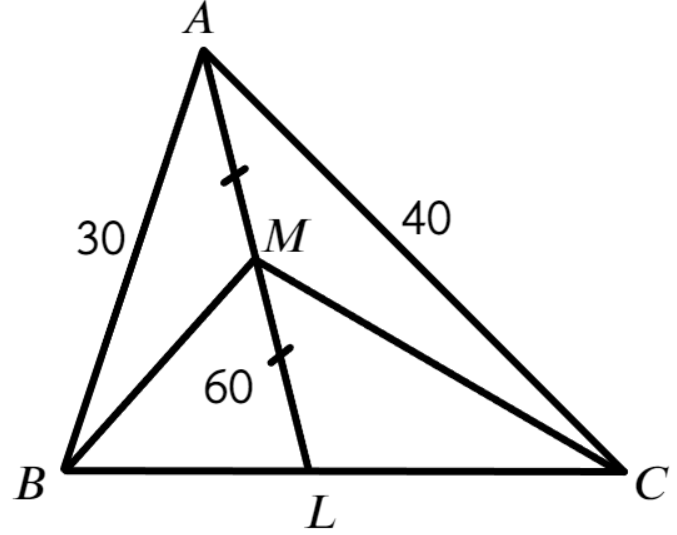
\includegraphics[scale=0.35]{g9-170.png}}
\end{figure}\\
Площади треугольников с общей высотой относятся так же, как основания, к которым она проведена. Поэтому $S_{\Delta ABM}=S_{\Delta BML}=60,\ S_{\Delta AMC}=S_{\Delta MLC}=x.$ Биссектриса делит основание в отношении, равном отношению прилежащих сторон, поэтому $\cfrac{BL}{LC}=\cfrac{30}{40}=\cfrac{3}{4}.$ Таким образом,
$\cfrac{S_{\Delta ABL}}{S_{\Delta ACL}}=\cfrac{BL}{LC}=\cfrac{3}{4},\ \cfrac{120}{2x}=\cfrac{3}{4},\ x=80.$\newpage\noindent
